\section{CHAD at First-Order}
\label{sec:first-order}

Our denotational approach to \GPS is based on the CHAD (Combinatory Homomorphic Automatic Differentiation) work of Mattias Vákár and others~\cite{vákár22,nunes2023}. Before we go into details, we present a high-level overview of their approach and how we have applied it to \GPS.

The fundamental approach in CHAD is to consider Grothendieck constructions on indexed categories $T : \cat{C}^\op \to \Cat$. An object of the Grothendieck construction $\int T$, described in more detail in \secref{Grothendieck}, is a pair $(X \in \cat{C}, \partial X \in T(X))$, which we read as pairing a space $X$ of ``points'' from $\cat{C}$ with an associated bundle of tangent spaces. The maps from the ``base'' category $\cat{C}$ are used to interpret the programs we are modelling. The maps in the indexed category are the maps of tangents or approximations, being derivatives and Galois connections respectively.

In the case of differentiable programs and automatic differentiation, a basic model can be constructed by taking $\cat{C}$ to be $\Set$ and $T(X) = X \to \FinVect$: indexed collections of finite dimensional vector spaces, whose elements are interpreted as tangents at the given point, with linear maps. The Grothendieck category $\int T$ has objects that are pairs of a set $X$ and for each $x \in X$ a tangent vector space $\partial X(x)$. Morphisms are pairs of maps of points to points, accompanied by linear maps of tangents at those points. If we carefully choose an initial set of maps, we can read these maps as derivatives (note that nothing in the Grothendieck construction says that they must be derivatives!). Composition in the Grothendieck category is exactly the {\em chain rule} for composing derivatives, so we at least do know that if we start with derivatives on basic operations, then composing them will retain this property.

For \GPS, we again take $\cat{C}$ to be $\Set$ and now take $T(X) = X \to \LatGal$: indexed collections of lattices, whose elements are interpreted as approximations at the given point, with indexed Galois connections as the maps between them.

In these special cases when $\cat{C} = \Set$, the Grothendieck construction is the {\em families} constructions $\Fam(\FinVect)$ and $\Fam(\LatGal)$~(\secref{Fam}). These settings are adequate for interpreting first-order programs, but neither is Cartesian closed. The picture for higher-order programs is more complicated. As is well known, $\Fam(\cat{X})$ for any category $\cat{X}$ is the free coproduct completion of $\cat{X}$~\cite{lawvere63}. In the case that $\cat{X}$ has a (symmetric) monoidal product, then we always get a symmetric monoidal product on $\Fam(\cat{X})$, using the Cartesian products from $\Set$. When $\cat{X}$ has all (small) products, and the monoidal product is actually a coproduct, then $\Fam(\cat{X})$ is symmetric monoidal closed. If the coproducts are actually {\em biproducts}~(\secref{biproducts}), then $\Fam(\cat{X})$ is Cartesian closed, and we can interpret higher-order programs.

Happily, $\FinVect$ and $\LatGal$ both have biproducts, as a consequence of their having products and being enriched in commutative monoids~(\propref{biproducts:from-product-or-coproduct} below). However, neither of them has all small products, without moving to infinite dimensional vector spaces (in the case of $\FinVect$) or complete lattices (in the case of $\LatGal$). Neither of these is ideal. In infinite dimensional vector spaces, dualisation is not involutive and the connection between the forward and reverse derivatives is lost. In complete lattices, we can no longer easily implement the infinite meets and joins required, and we lose the computability of the model. Moreover, in Agda, there are issues with predicativity when considering complete lattices. \todo{be more specific}

Vákár and collaborators overcome this by using different interpretations for forward and backward derivatives. We overcome this by using $\CMon$-enriched presheaves, as described in \secref{higher-order}; first we present a suitable first-order setting.

\subsection{$\CMon$-Categories and Biproducts}
\label{sec:biproducts}

\subsubsection{$\CMon$-Categories}

A category $\cat{C}$ is enriched in $\CMon$, the (monoidal) category of commutative monoids, if every hom-set
$\cat{C}(X,Y)$ provides an operation + to add morphisms together, as well as a zero morphism $0: X \to Y$, and
composition is \emph{bilinear}, i.e.~given by a family of morphisms $\Hom{\cat{C}}{Y}{Z} \tensor
\Hom{\cat{C}}{X}{Y} \to \Hom{\cat{C}}{X}{Z}$ in $\CMon$ that preserve the additive structure in
$\Hom{\cat{C}}{Y}{Z}$ and $\Hom{\cat{C}}{X}{Y}$ separately:

\begin{salign*}
f \comp \zero = f = \zero \comp f
\end{salign*}
\begin{salign*}
(f + g) \comp h &= (f \comp h) + (g \comp h) \\
h \comp (f + g) &= (h \comp f) + (h \comp g)
\end{salign*}

In a $\CMon$-category, any products and coproducts coincide.

\begin{proposition}
\label{prop:biproducts:from-product-or-coproduct}
In any $\CMon$-category:
\begin{enumerate}
\item If $X \times Y$ is a product then it is also coproduct, with $\inj_1 = \prodM{\id}{0}$ and $\inj_2 =
\prodM{0}{\id}$.
\item If $X \coprod Y$ is a coproduct then it is also a product, with $\pi_1 = \coprodM{\id}{0}$ and $\pi_2 =
\coprodM{0}{\id}$.
\item $X$ is terminal iff it is initial.
\end{enumerate}
\end{proposition}

An object that is both terminal and initial is called a \emph{zero} object; an object that is both a product
and a coproduct is called a \emph{biproduct}.

\subsubsection{Biproducts}

More directly, a biproduct is as an object $X \biprod Y$ together with morphisms

\begin{center}
\begin{tikzcd}
   X \arrow[r, "\biinj_X", shift left] &
   X \biprod Y \arrow[l, "\biproj_X", shift left] \arrow[r, "\biproj_Y"', shift right] &
   Y \arrow[l, "\biinj_Y"', shift right]
\end{tikzcd}
\end{center}

\noindent satisfying

\vspace{-3mm}
\begin{minipage}[t]{0.45\textwidth}
\begin{center}
\begin{salign*}
   \biproj_X \comp \biinj_X &= \id_X \\
   \biproj_Y \comp \biinj_X &= \zero_{X,Y}
\end{salign*}
\end{center}
\end{minipage}%
\begin{minipage}[t]{0.45\textwidth}
\begin{center}
\begin{salign*}
   \biproj_Y \comp \biinj_Y &= \id_Y \\
   \biproj_X \comp \biinj_Y &= \zero_{Y,X}
\end{salign*}
\end{center}
\end{minipage}

\begin{salign*}
(\biinj_X \comp \biproj_X) + (\biinj_Y \comp \biproj_Y) &= \id_{X \biprod Y}
\end{salign*}

\noindent from which the universal properties of the product and coproduct easily follow. A category $\cat{C}$
with finite biproducts is called \emph{semi-additive}. A semi-additive category cannot be Cartesian closed
without being trivial: since we have $X \iso 0 \biprod X$, Cartesian closure would imply $\Hom{\cat{C}}{X}{Y}
\iso \Hom{\cat{C}}{0}{X \Rightarrow Y} \iso 1$, and therefore in such a category all objects are isomorphic.

% in any such category the canonical projections and injections give an isomorphism $\textstyle X \coprod Y
% \iso X \times Y$ that is natural in both variables
%
% A semi-additive category $\cat{C}$ is enriched in $\CMon$: for any two morphisms $f, g: X \to Y$ in
% $\cat{C}$, the biproduct structure provides a way to ``add'' them together, forming a morphism $f + g: X \to
% Y$. Diagrammatically:
%
% \begin{center} \begin{tikzcd} X \arrow[r, "\diag"] & X \biprod X \arrow[r, "f \biprod g"] & Y \biprod Y
% \arrow[r, "\codiag"] & Y \end{tikzcd} \end{center}
%
% Here $\diag$ denotes the diagonal $\prodM{\id_X}{\id_X}$ given by the universal property of the product and
% $\codiag$ denotes the codiagonal $\coprodM{\id_X}{\id_Y}$ given by the universal property of the coproduct.
% The $f \oplus g$ morphism is the component-wise map $\prodM{f \comp \biproj_X}{g \comp \biproj_Y} =
% \coprodM{\biinj_X \comp f}{\biinj_Y \comp g}$. Similarly we can exhibit a \emph{zero} morphism $0_{X,Y}$ by
% composing the unique maps in and out of the zero object:
%
% \begin{center} \begin{tikzcd} X \arrow[r, "!_X"] & 0 \arrow[r, "!^Y"] & Y \end{tikzcd} \end{center}
%
% It is easy to verify that $+$ is associative and commutative and that $f + 0_{X,Y} = f$, and thus that every
% hom-object $\cat{C}(X,Y)$ is an object in $\CMon$.
%
% \subsubsection{Biproduct laws}
%
% It is also possible to use these laws to define biproducts, in the case where $\cat{C}$ is enriched in
% $\CMon$ and so equipped with addition of morphisms and zero morphisms. In that case any products or
% coproducts in $\cat{C}$ are necessarily biproducts.

\subsubsection{Example: Category of Finite Vector Spaces}
\label{sec:categories-with-biproducts:fdvect}

The category $\FinVect$ of finite vector spaces over $\RR$ is semi-additive.

\begin{definition}
Define $\FinVect$ to be the category which has as objects $\RR^n$ all finite-dimensional vector spaces
$(\RR^n, +, \mult)$, and as morphisms $f: \RR^m \to \RR^n$ all functions $f$ satisfying $f(u + v) = f(u) +
f(v)$ and $f(a \mult v) = a \mult f(v)$.
% with $f$ preserving the zero and additive inverse structure automatically.
\end{definition}

%  with addition of real numbers written $a + b$ and multiplication written $a \mult b$

% \begin{definition}[Finite dimensional vector space over $\RR$]
% Up to isomorphism, an \emph{$n$-dimensional vector space over $\RR$} is the set $\RR^n$ equipped with
% component-wise addition of vectors and scalar multiplication (also written $+$ and $\mult$), where $(\RR^n,+)$
% is an abelian group (with identity $0$ and additive inverse $-v$ again defined component-wise), and where the
% vector operations are compatible with the field operations in that the following equations hold:
%
% \vspace{-4mm}
% \begin{minipage}[t]{0.45\textwidth}
% \begin{center}
% \begin{align*}
%    1 \mult v &= v \\
%    (a \mult b) \mult v &= a \mult (b \mult v)
% \end{align*}
% \end{center}
% \end{minipage}%
% \begin{minipage}[t]{0.45\textwidth}
% \begin{center}
% \begin{align*}
%    (a + b) \mult v &= (a \mult v) + (b \mult v) \\
%    a \mult (u + v) &= (a \mult u) + (b \mult v)
% \end{align*}
% \end{center}
% \end{minipage}
% \end{definition}

$\FinVect$ is enriched in $\CMon$ (in fact in $\Ab$, the category of abelian groups, but $\CMon$ will do for
our purposes). For any objects $V = \RR^m$ and $W = \RR^n$, the hom-set $\FinVect(V,W)$ provides pointwise
addition of morphisms $(f + g)(v) = f(v) + g(v)$; the constant map $v \mapsto 0$ is a zero morphism, and
composition is bilinear. Moreover the direct sum $V \biprod W \iso \RR^{m + n}$ given by the Cartesian product
is a biproduct, with $\biinj_{V} = \prodM{\id}{0}$ and $\biinj_{W} = \prodM{0}{\id}$.

\subsubsection{Example: Category of Lattices and Galois Connections}

The category $\LatGal$ of bounded lattices and Galois connections is semi-additive.

\begin{definition}[Galois connection]
A \emph{Galois connection} $f \adj g: X \to Y$ is a pair of monotone functions $f: Y \to X$ and $g: X \to Y$
between posets satisfying $y \leq g(x) \iff f(y) \leq x$.
\end{definition}

\noindent A Galois connection $f \adj g: X \to Y$ is an adjunction between poset categories, regarding
monotone $f$ and $g$ as functors; $f$ is usually referred to as the \emph{upper} (right) adjoint and $g$ as
the \emph{lower} (left) adjoint. Galois connections are closed under component-wise composition and identities
$\id_X \adj \id_X$.

\begin{definition}
Define $\LatGal$ to be the category which has as objects $X = (X, \meet, \join, \top, \bot)$ all bounded
lattices, and as morphisms all Galois connections $f \adj g: X \to Y$.
\end{definition}

\noindent Since right adjoints preserve limits and left adjoints preserve colimits, for any $f \adj g: X \to
Y$ we have that $g$ preserves the meet-semilattice structure $(X, \meet, \top)$, and similarly $f$ preserves
the join-semilattice structure $(X, \join, \bot)$. The meet-preserving maps are enriched in $\CMon$ (in fact
in $\SemiLat$, but again $\CMon$ is sufficient): addition of maps is computed pointwise via $\meet$, since $(f
\meet g)(x) = f(x) \meet g(x)$ preserves meets, with the constant map $\top = x \mapsto \top_Y$ as a zero.
Dually the join-preserving maps can be added pointwise using $\join$, with the constant map $\bot = y \mapsto
\bot_X$ as a zero. Since these constructions come in adjoint pairs, $\LatGal$ is enriched in $\CMon$. The
hom-set $\LatGal(X,Y)$ provides (component-wise) addition of Galois connections $(f \adj g) + (f' \adj g') =
(f \join f') \adj (g \meet g')$; the Galois connection $\bot \adj \top$ is a zero morphism, and composition is
bilinear.

$\LatGal$ also has biproducts. The projections $\pi_1$ and $\pi_2$ from the product lattice $X \times Y$ have
both upper and lower adjoints; this means that $X \times Y$ (which we shall write as $X \biprod Y$), is both a
product and a coproduct, with projections $\biproj_X$ and $\biproj_Y$ and injections $\biinj_X$ and $\biinj_Y$
given by:

\vspace{-4mm}
\begin{minipage}[t]{0.45\textwidth}
\begin{center}
\begin{align*}
   \biproj_X = \prodM{\id}{\bot} \adj \proj_1: X \biprod Y \to X \\
   \biproj_Y = \prodM{\bot}{\id} \adj \proj_2: X \biprod Y \to Y
\end{align*}
\end{center}
\end{minipage}%
\begin{minipage}[t]{0.45\textwidth}
\begin{center}
\begin{align*}
   \biinj_X = \pi_1 \adj \prodM{\id}{\top} : X \to X \biprod Y \\
   \biinj_Y = \pi_2 \adj \prodM{\top}{\id}: Y \to X \biprod Y
\end{align*}
\end{center}
\end{minipage}
\vspace{2mm}

\noindent with the trivial 1-point lattice as a zero object (terminal and initial).

\subsection{Grothendieck Construction for Indexed Categories}
\label{sec:Grothendieck}

We now consider how to adapt the CHAD framework~\cite{vákár22,nunes2023} to interpret programs as functions
along with their forward and backward approximation maps. Since the appropriate lattice of approximation
typically depends on the value being approximated, we will want to interpret a type $\tau$ as a pair $(X,
\partial X)$ where $X$ provides the conventional interpretation as a set and $\partial X$ provides an
appropriate lattice of approximations $\partial X(x)$ for every point $x \in X$. An expression $e$ of type
$\sigma$ with a single free variable of type $\tau$ (supposing $\tau$ and $\sigma$ denote $X$ and $Y$ in the
conventional semantics) must then be interpreted by a pair $(f, \partial f)$, with $f$ providing the
conventional interpretation as a function $X \to Y$, and $\partial f$ as a family of Galois connections
$\partial f(x): \partial X(x) \to \partial Y(f(x))$ taking approximants to approximants.

This pattern of objects and morphisms is captured by the construction used in CHAD to model automatic
differentiation, namely the \emph{Grothendieck construction} for a particular set-indexed category $T:
\Set^\op \to \Cat$. For automatic differentiation, $T(X)$ will be the functor category $\Func{X}{\FinVect}$,
regarded as the category of $X$-indexed families of finite vector spaces, with families of linear maps as
morphisms. For Galois slicing, we will take $T(X) = \Func{X}{\LatGal}$, the category of $X$-indexed families
of bounded lattices, with families of Galois connections as morphisms.

In its general form, the Grothendieck construction $\Grothendieck{}T$ for an arbitrary indexed category $T:
\cat{C}^\op \to \Cat$, sometimes called the \emph{total category} for $T$, incorporates all the categories
$T(X)$ (for objects $X$ in $\cat{C}$) into a single category, together with morphisms that account for both
internal structure and reindexing along morphisms $f: X \to Y$ in $\cat{C}$.

\begin{definition}
\label{def:Grothendieck}
Suppose $T: \cat{C}^\op \to \Cat$ an indexed category. The \emph{Grothendieck construction}
$\Grothendieck{X}T(X)$ (also written $\Grothendieck{}T$) is the category which has as objects, all pairs $(X,
\partial X)$ of an object $X$ of $\cat{C}$ and an object $\partial X$ of $T(X)$, and as morphisms $(X,
\partial X) \to (Y, \partial Y)$, all pairs $(f, \partial f)$ of morphisms $f: X \to Y$ in $\cat{C}$ and
morphisms $\partial f: \partial X \to T(f)(\partial Y)$ in $T(X)$.
\end{definition}

\noindent The $\partial X$ notation is intended to suggest the connection between the Grothendieck
construction and the idea of tangent spaces and derivatives. For any $(f, \partial f): (X, \partial X) \to (Y,
\partial Y)$ and $(g, \partial g): (Y, \partial Y) \to (Z, \partial Z)$ in $\Grothendieck{}T$, the composition
$(g, \partial g) \comp (f, \partial f): (X, \partial X) \to (Z, \partial Z)$ is given by $(g \comp f,
T(f)(\partial g) \comp \partial f)$, with the functor $T(f)$ acting to ``reindex'' $\partial g$ along $f$,
yielding a morphism $T(f)(\partial g): T(f)(\partial Y) \to T(f)(T(g)(\partial Z)) = T(g \comp f)(\partial
Z)$.

\subsubsection{Category of Families}
\label{sec:Fam}

For CHAD we are interested in the specific case of the Grothendieck construction where $\cat{C} = \Set$ and
each category $T(X) = \Func{X}{\cat{C}}$, the functor category which has as objects all $X$-indexed families
of objects of $\cat{C}$, and as morphisms $F \to G$, all families of morphisms $\eta(x): F(x) \to G(x)$ in
$\cat{C}$ (with naturality trivial because $X$ has only identity morphisms).

% Like any functor category $\Func{X}{\cat{C}}$ inherits limits and colimits pointwise from its codomain.
%
% \begin{proposition}
% If $\cat{C}$ has limits (resp.~colimits) then $\Func{X}{\cat{C}}$ has limits (resp.~colimits) computed
% pointwise.
% \end{proposition}

\begin{definition}[Reindexing]
For any function $f: X \to Y$ define the \emph{reindexing} functor $\reindex{-}{f} = \Func{f}{\cat{C}}:
\Func{Y}{\cat{C}} \to \Func{X}{\cat{C}}$ which sends any $Y$-indexed family $F$ over $\cat{C}$ to the
$X$-indexed family $\reindex{F}{f} = F \comp f$ (regarding $f$ as a functor between $X$ and $Y$ as discrete
categories) and any family of morphisms $\eta: F \to G$ to $\reindex{\eta}{f}: \reindex{F}{f} \to
\reindex{G}{f}$ with $\reindex{\eta}{f}(x) = \eta(f(x))$.
\end{definition}

\noindent Although reindexing is just precomposition with $f$, writing it as $\reindex{-}{f}$ avoids
notational confusion when combining composition of morphisms in $\Func{X}{C}$ with reindexing.

The Grothendieck construction for $\Func{-}{\cat{C}}: \Set^{\op} \to \Cat$, the indexed category which sends
any set $X$ to the category of indexed families $\Func{X}{\cat{C}}$ and any function $f: X \to Y$ to the
reindexing functor $\reindex{-}{f}: \Func{Y}{\cat{C}} \to \Func{X}{\cat{C}}$, is called the \emph{families}
construction for $\cat{C}$.

\begin{definition}[Categories of families]
\label{def:Fam}
For any category $\cat{C}$ define $\Fam(\cat{C})$ to be the Grothendieck construction
$\Grothendieck{X}\Func{X}{\cat{C}}$.
\end{definition}

\noindent In $\Fam(\cat{C})$ the objects $(X, \partial X)$ are thus all pairs of sets $X$ and indexed families
$\partial X: X \to \cat{C}$ and the morphisms $(f, \partial f): (X, \partial X) \to (Y, \partial Y)$ are all
pairs of functions $f: X \to Y$ and morphisms $\partial f: \partial X \to \partial \reindex{Y}{f}$ in
$\Func{X}{\cat{C}}$.

\begin{proposition}
\label{prop:Grothendieck:fam-inherits-local-smallness}
If $\cat{C}$ is locally small then so is $\Fam(\cat{C})$.
\end{proposition}

\begin{proposition}
\label{prop:Grothendieck:fam-inherits-products}
If $\cat{C}$ is (symmetric) monoidal then $\Fam(\cat{C})$ is also (symmetric) monoidal, with tensor product
$(X, \partial X) \tensor (Y, \partial Y) = (X \times Y,(x, y) \mapsto \partial X(x) \tensor \partial Y(y))$.
\end{proposition}

\subsection{First-Order Galois Slicing via CHAD}
\label{sec:fam:galois-slicing}

The total category $\Fam(\LatGal)$ is then a suitable setting for interpreting first-order programs for \GPS.
It has as objects $(X, \partial X)$, all pairs of a set $X$ and and for every $x \in X$, a bounded lattice
$\partial X(x)$, and as morphisms $(X, \partial X) \to (Y, \partial Y)$, all pairs $(f, \partial f)$ of a
function $f: X \to Y$ and for every $x \in X$, a Galois connection $\partial f(x): \partial X(x) \to \partial
Y(f(x))$. The reindexing along $f$ in the composition $(g, \partial g) \comp (f, \partial f) = (g \comp f,
\reindex{\partial g}{f} \comp \partial f)$ selects the appropriate lattice of approximations and Galois
connection at each point, using the baseline (unapproximated) function $f$.

For a first-order language with a primitive type $\syn{nat}$ and primitive operations such as $+$, the
language would provide a model of $\syn{nat}$ and its operations in $\Fam(\LatGal)$. For example, we might
interpret $\syn{nat}$ as the object $(\Nat,n \mapsto \downset{n})$, where the family component assigns to
every natural number $n$ the two-point lattice $\downset{n} = \{n, \bot\}$ indicating whether $n$ is fully
present ($n$) or fully absent ($\bot$) from an approximation of $n$, as shown in the example in
\secref{introduction}. A slight variant is to use the constant family which assigns to every $n$ the two-point
lattice $\Two = \{\mathsf{tt},\mathsf{ff}\}$; using $\downset{n}$ can be more useful in practice as the
approximants of a given value then contain all the information about the value that hasn't been approximated
away.

We might interpret $+$ as the morphism $(+,\partial+)$, i.e.~the usual addition operator + paired with an
approximating version $\partial+_{n,m}: \downset{n} \to \downset{m}$ defined as:
\begin{displaymath}
    \begin{array}[t]{l@{(}l@{,~}l@{)~}c@{~}l}
      \partial+_{n,m}&n&m&=&n + m \\
      \partial+_{n,m}&\bot&\_&=&\bot \\
      \partial+_{n,m}&\_&\bot&=&\bot
    \end{array}
\end{displaymath}
These elementary approximation structures would then be combined by the interpretation of composite types like
sums and products, providing suitable derived structures for composite values.

\subsubsection{Lifting}

A programmer, or perhaps a language implementor, might want to embed additional ``approximation points'' into
composite data types, to allow for richer approximation structures. For example, for a list like $1 : 2 : []$
we might want to allow the partial lists $\bot$, $1 : \bot$ and $1 : 2 : \bot$ as approximants, in addition to
the approximants obtained by replacing elements with $\bot$. This can be accomplished by extending the syntax
with a \emph{lifting} type constructor $\tyLift$. Then, as an alternative to the usual definition of lists of
natural numbers as $\mu\alpha.1 + \synVar{nat} \times \alpha$, one could (within the language) define a type
of ``approximation lists'' $\mu\alpha.\tyLift\,(1 + \tyLift\,\synVar{nat} \times \alpha)$, with monadic
computations over approximated lists computing partial lists like $1 : \bot$. The lattice of approximants of
$1 : 2 : []$ now includes not only all the ``shape-preserving'' approximations but also all prefixes obtained
by truncating successive tails with $\bot$:

  \begin{center}
    \tikzset{node distance=1cm}
    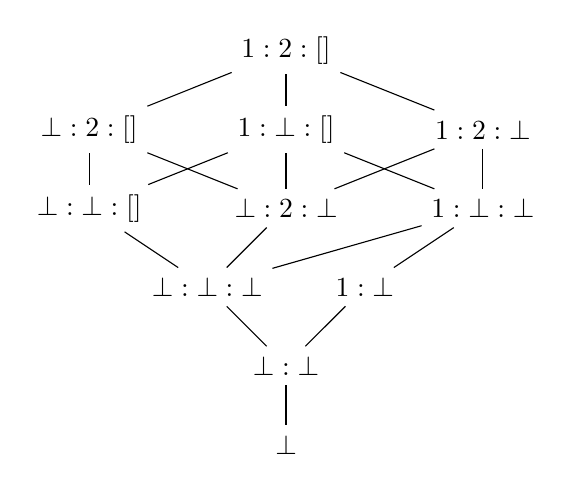
\begin{tikzpicture}
      \node (top) at (0,0) {$1 : 2 : []$};
      % row 2
      \node [below of=top] (ioi) {$1 : \bot : []$};
      \node [left of=ioi,xshift=-1.5cm] (oii) {$\bot : 2 : []$};
      \node [right of=ioi,xshift=1.5cm] (iio) {$1 : 2 : \bot$};
      % row 3
      \node [below of=ioi] (oio) {$\bot : 2 : \bot$};
      \node [left of=oio,xshift=-1.5cm] (ooi) {$\bot : \bot : []$};
      \node [right of=oio,xshift=1.5cm] (ioo) {$1 : \bot : \bot$};
      % row 4
      \node [below of=oio,xshift=-1cm] (ooo) {$\bot : \bot : \bot$};
      \node [below of=oio,xshift=1cm] (io) {$1 : \bot$};
      % row 5
      \node [below of=ooo,xshift=1cm] (oo) {$\bot : \bot$};
      % row 6
      \node [below of=oo] (o) {$\bot$};

      % links
      \draw (top) -- (ioi);
      \draw (top) -- (oii);
      \draw (top) -- (iio);
      \draw (ioi) -- (oio);
      \draw (ioi) -- (ooi);
      \draw (ioi) -- (ioo);
      \draw (oii) -- (oio);
      \draw (oii) -- (ooi);
      \draw (iio) -- (oio);
      \draw (iio) -- (ioo);
      \draw (ooi) -- (ooo);
      \draw (oio) -- (ooo);
      \draw (ioo) -- (ooo);
      \draw (ioo) -- (io);
      \draw (ooo) -- (oo);
      \draw (io) -- (oo);
      \draw (oo) -- (o);
    \end{tikzpicture}
  \end{center}

Similarly, one could define a custom approximating version of multiplication $*_{\text{appr}}:
\tyLift\,\synVar{nat} \times \tyLift\,\synVar{nat} \to \tyLift\,\synVar{nat}$, as:
\[x *_{\text{appr}} y = \tmBind{x}{\tmFun{x'}{\syn{if}\;x' \equiv
0\;\syn{then}\;\tmReturn{0}\;\syn{else}\;\tmBind{y}{\tmFun{y'}{\tmReturn{x' * y'}}}}}\]

\noindent This would allow the programmer to emulate the short-circuiting behaviour of $\mathrm{strictOr}$
from \exref{strict-short-circuit}, or the short-circuiting multiplication used in \citet{perera22} for slicing
matrix convolutions, without having to bake specific choices of approximation into the interpretation of
individual operators.

With this lifting operator in the core language, one could then choose to fix certain choices of
approximation, providing a surface language without the lifting monad and interpreting it into the core
language with lifting. The Galois slicing implementations discussed in \citet{perera12a} and
\citet{ricciotti17}, for example, provide an approximation point at every composite type constructor; we can
emulate this in our approach by defining a surface language where the data type of lists $\mu\alpha.1 +
\synVar{nat} \times \alpha$ desugars automatically into the approximating version $\mu\alpha.\tyLift\,(1 +
\tyLift\,\synVar{nat} \times \alpha)$.

To interpret the syntactic type constructor $\tyLift$, consider the strong monad $(\Lift, \eta, \mu)$ which
acts on a poset $X$ to extend it with a distinguished bottom element $\bot$ and on a monotone function $f$
between posets to extend it with a mapping from $\bot$ to $\bot$. $\Lift$ is also a strong monad on
meet-semilattices. On (bounded) join-semilattices, $\Lift$ induces a costrong comonad $(\Lift, \varepsilon,
\delta)$, with the bottom element of $X$ needed to implement the counit $\varepsilon_X: \Lift(X) \to X$. These
two combine to form a strong lifting monad in $\LatGal$ with unit $\varepsilon_X \dashv \eta_X$ and
multiplication $\delta_X \dashv \mu_X$.

The lifting monad $\Lift$ in $\LatGal$ is preserved into $\Fam(\LatGal)$. The families construction, regarded
as a covariant 2-functor $\Fam(-): \Cat \to \Cat$, sends functors $F: \cat{C} \to \cat{D}$ to functors
$\Fam(F): \Fam(\cat{C}) \to \Fam(\cat{D})$ that reassign the target category by postcomposing with $F$,
sending objects $(X, \partial X)$ to $(X, F \comp \partial X)$ and morphisms $(f, \partial f)$ to $(f, F \comp
\partial f)$, where $F \comp \partial f$ denotes the natural transformation where $(F \comp \partial f)(x) =
F(\partial f(x))$. If $F$ happens to be a (strong) monad on $\cat{C}$, then $\Fam(F)$ is a (strong) monad on
$\Fam(\cat{C})$, computed by extending the original monad $F: \cat{C} \to \cat{C}$ componentwise to families.

\subsection{First-Order Automatic Differentiation via CHAD}
\label{sec:first-order:autodiff}

As per the CHAD work, automatic differentiation (AD) for first-order programs can also be recovered in this
setup, using the total categories $\Fam(\FinVect)$ and $\Fam(\FinVect^\op)$ instead of $\Fam(\LatGal)$. First
we recall the chain rule for forward derivatives $\pushf{f}_x: \RR^m \linearto \RR^n$ and backward derivatives
$\pullf{f}_x: \RR^n \linearto \RR^m$, which says that derivatives respect composition~\cite{spivak65}.

% \subsubsection{Derivatives of Differentiable Functions}
%
% For flat manifolds like $\RR^n$, the tangent space and cotangent space at a point $x$ are both canonically
% isomorphic to $\RR^n$, so the forward and backward derivatives of a differentiable function $f: \RR^m \to
% \RR^n$ at a point $x$ have the following form \todo{Can probably delete now as covered in
% \secref{approx-as-tangents}}:
%
% \begin{itemize}
% \item The \emph{forward derivative} (tangent map or pushforward) $\pushf{f}_x$ of $f$ at $x \in \RR^m$ is the
% unique linear map $\RR^m \linearto \RR^n$ given by the Jacobean matrix of $f$ at $x$.
% \item The \emph{backward derivative} (cotangent map or pullback) $\pullf{f}_x$ is the unique linear map
% $\RR^n \linearto \RR^m$ given by the transpose (adjoint) of the Jacobean matrix of $f$ at $x$.
% \end{itemize}

\begin{proposition}[Chain Rule]
Suppose $f: \RR^m \to \RR^n$ and $g: \RR^n \to \RR^k$ differentiable. Then for any $x \in \RR^m$ we have:

\begin{itemize}
\item $\pushf{(g \comp f)}_x = \pushf{g}_{f(x)} \comp \pushf{f}_x: \RR^m \to \RR^k$
\item $\pullf{(g \comp f)}_x = \pullf{f}_{x} \comp \pullf{g}_{f(x)}: \RR^k \to \RR^m$
\end{itemize}
\end{proposition}

\subsubsection{Automatic Differentiation}

The basic idea of (forward-mode) AD, as first described by \citet{linnainmaa76}, was to recognise that one
could efficiently compute the pushforward map $\pushf{f}: \RR^m \to (\RR^m \linearto \RR^n)$ of a
differentiable function $f: \RR^m \to \RR^n$ alongside the computation of $f$ itself, by defining a single map
$\tangents(f) = x \mapsto (f(x), \pushf{f}_x): \RR^m \to \RR^n \times (\RR^m \linearto \RR^n)$. Writing $g_1$
for $\pi_1 \comp g$ and $g_2$ for $\pi_2 \comp g$, composition of such maps can be expressed as:
\begin{align*}
(g \comp h)_1(x) &= g_1(h_1(x)) \\
(g \comp h)_2(x) &= g_2(h_1(x)) \comp h_2(x)
\end{align*}

We can verify that $\tangents$ is functorial, regardless of whether the linear maps happen to be derivatives.
But if $h_2(x)$ is the derivative of $h_1$ at $x$ for any $x \in \RR^m$ and similarly for $g$ then the
derivatives compose according to the forward chain rule and $(g \comp h)_2(x)$ is the derivative of $(g \comp
h)_1$ at $x$. Thus this setup provides an algorithmic method for computing the forward derivative of a
composite function, as long as all atomic operations provide derivatives, without have to recompute the
function itself.

% An efficient implementation of \GPS based on $\Fam(\LatGal)$
% (\secref{fam:galois-slicing} above) would most likely apply a similar optimisation to make it possible to
% compute forwards slices without having to reexecute the program at the same time.

We can see these ``optimised'' forward-mode maps as living in $\Fam(\FinVect)$ if we regard every finite
vector space $\RR^n$ as paired with the family of tangent spaces which is constantly $\RR^n$, and each map $g:
\RR^m \to \RR^n \times (\RR^m \linearto \RR^n)$ as a pair of maps $(g_1, g_2)$. Then the composition $(g,
\partial g) \comp (h, \partial h) = (g \comp h, \reindex{\partial g}{h} \comp \partial h)$ again corresponds
to the forward chain rule, since $(\reindex{\partial g}{h} \comp \partial h)_x = {\partial g}_{h(x)} \comp
{\partial h}_x$. Analogously, reverse-mode maps $g: \RR^m \to \RR^n \times (\RR^n \linearto \RR^m)$ can be
interpreted as living in $\Fam(\FinVect^\op)$ by reading them as pair of maps $(g_1, g_2)$ with composition
being precisely the backwards chain rule.
